\documentclass[a4paper, 12pt]{article}

\usepackage[top=2cm, bottom=2cm, left=2.5cm, right=2.5cm]{geometry}
\usepackage[utf8]{inputenc}
\usepackage{array}
\usepackage{verbatim}
\usepackage{graphicx}
\usepackage{hyperref}

\graphicspath{{img/}}

\begin{document}

\includegraphics{logo}\\
\textbf{UNIVERSIDADE ESTADUAL DE PONTA GROSSA} \\
SISTEMA UNIVERSIDADE ABERTA DO BRASIL - UAB \\
\underline{Licenciatura em Matemática | Polo UAB em Jacarezinho} \\
\textbf{ALUNO:} Ricardo Medeiros da Costa Junior   \textbf{RA:} 151774301 \\
\textbf{DISCIPLINA:} Instrumentação para o Ensino da Matemática IV \\
\textbf{ATIVIDADE:} Atividade 5 - Tarefa Descritiva (Valor: 5,0) \\

\begin{enumerate}
\item Analise os problemas matemáticos apresentados abaixo, tendo como referencial teórico o texto postado na unidade II: \textbf{“O ensino de matemática proposto nos PCN+ Ensino Médio e nas Diretrizes Curriculares da SEED/PR”}, quanto aos itens apresentados no quadro abaixo de cada questão.(Questões retiradas nas Olimpíadas de Matemática)
\begin{figure}[h!]
  \centering
  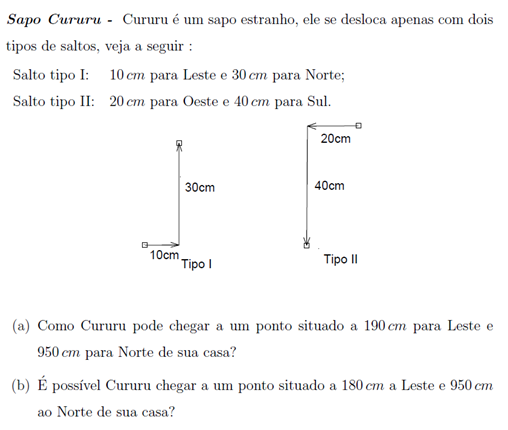
\includegraphics[width=0.5\textwidth]{1}
\end{figure} 
  \begin{enumerate}
  \item Eixo estruturante (PCN e DCE)\\\\
    PCN: Geometria e Medidas\\
    DCE: Geometria
  \item Conteúdo Matemático (Ensino Médio) \\\\
    PCN: Geometria Analítica\\
    DCE: Geometria Analítica
  \item Conhecimentos matemáticos necessários para resolvê-la \\\\
    O aluno terá que saber transformar problemas geométricos em equações e resolvê-la.
  \item Presença ou não da interdisciplinaridade \\\\
    Sim, pois é necessário saber temas como equações e álgebra para poder abstrair o que o exercício pede.
  \item Presença de contextualização no texto da questão\\\\
    Sim, porque é explicado claramente no enunciado do exercício o que é solicitado.
  \end{enumerate}

\begin{figure}[h!]
  \centering
  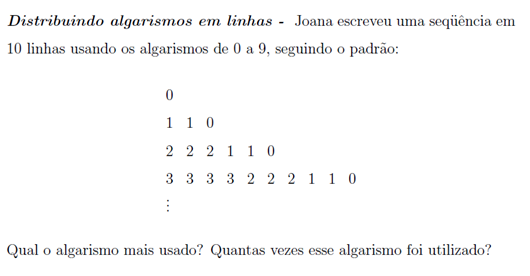
\includegraphics[width=0.5\textwidth]{2}
\end{figure} 
  \begin{enumerate}
  \item Eixo estruturante (PCN e DCE)\\\\
    PCN: Álgebra: Números e Funções\\
    DCE: Números e Funções
  \item Conteúdo Matemático (Ensino Médio) \\\\
    PCN: Sequências\\
    DCE: Números reais
  \item Conhecimentos matemáticos necessários para resolvê-la \\\\
    O aluno deve se ater à lei de formação dessas sequência e conseguir associar ao problema.
  \item Presença ou não da interdisciplinaridade \\\\
    Não, apenas o conteúdo matemático de números e funções.
  \item Presença de contextualização no texto da questão\\\\
    Sim, porque é possível entender o que o exercício pede.
  \end{enumerate}
\begin{figure}[h!]
  \centering
  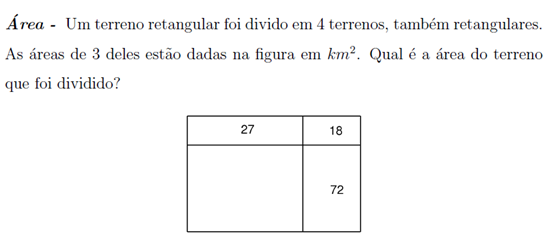
\includegraphics[width=0.5\textwidth]{3}
\end{figure} 
  \begin{enumerate}
  \item Eixo estruturante (PCN e DCE)\\\\
    PCN: Geometria e Medidas\\
    DCE: Geometrias
  \item Conteúdo Matemático (Ensino Médio) \\\\
    PCN: Geometria Plana \\
    DCE: Geometria Plana; Medidas de área
  \item Conhecimentos matemáticos necessários para resolvê-la \\\\
    Interpretação de problemas geométricos. Abstração algébrica; Cálculo de área de figuras planas    
  \item Presença ou não da interdisciplinaridade \\\\
    Não é solicitado apenas conteúdo de geometria plana
  \item Presença de contextualização no texto da questão\\\\
    Sim, pelo enunciado do exercício é possível interpretar claramente.
  \end{enumerate}
\begin{figure}[h!]
  \centering
  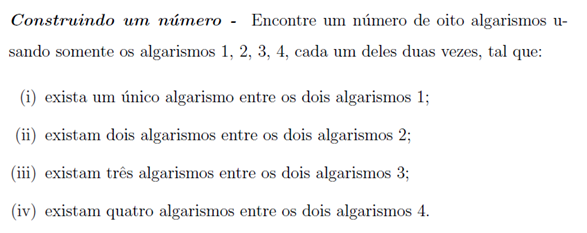
\includegraphics[width=0.5\textwidth]{4}
\end{figure} 
  \begin{enumerate}
  \item Eixo estruturante (PCN e DCE)\\\\
    PCN: Análise de dados \\
    DCE: Tratamento de Informação
  \item Conteúdo Matemático (Ensino Médio) \\\\
    PCN: Contagem\\
    DCE: Análise combinatória   
  \item Conhecimentos matemáticos necessários para resolvê-la \\\\
    Desenvolver o raciocínio combinatório. Ou seja, decidir sobre a forma mais adequada de organizar números ou informações para poder contar os casos possíveis
  \item Presença ou não da interdisciplinaridade \\\\
    Sim, pois é necessário usar conteúdo do eixo de números também
  \item Presença de contextualização no texto da questão\\\\
    Sim, pelo enunciado do exercício é possível interpretar claramente.
  \end{enumerate}
\end{enumerate}
\end{document}
